\documentclass[authoryear, 12pt,5p, times]{elsarticle}
%\usepackage[hypcap]{caption}
%\geometry{margin=0.95in,top=1.4in,bottom=1.4in}
\geometry{margin=1in,top=1.3in,bottom=1.3in}
\usepackage{float}
\usepackage{amsmath}
\usepackage[hidelinks]{hyperref} 
 \usepackage{gensymb}
\usepackage{subcaption}
\usepackage{url}
%\renewcommand\thefootnote{\fnsymbol{\dagger}}
\usepackage[symbol*]{footmisc}
\newcommand{\rpm}{\raisebox{.2ex}{$\scriptstyle\pm$}}
\begin{document}
%\footnote{This is a footnote}
\begin{frontmatter}
\title{Asteroid Astrometry from CCD Images}
\author{\today \\ \quad \\Jung Lin (Doris) Lee\\ dorislee@berkeley.edu\\Group partners: Jennifer Ito, Manuel Silvia\\Prof. James Graham, UGSI Heechan Yuk, Isaac Domagalski}
	\begin{abstract}
In this experiment,  we------
	\end{abstract}
\end{frontmatter}
\section{Introduction}
Distance is undoubtedly one of the most important but hard to measure quantities in astronomy. Distance is necessary for deriving the Keplerian orbital elements, luminosity, true motion, size and mass of the astronomical object for detailed studies of origin, structure and evolutionary history of our Galaxy. However, due to the enormity of astronomical length scales, astronomical distances can not be directly measured but can be inferred from using the method of parallax. The idea of using parallax for astrometry has been around for more than two thousand years, but most attempts had been fruitless due to instrument constraints on the telescopes resolution or the naked eye. Recent space missions such as Gaia (Lindegren et al.) and  Hipparcos (Perryman et al.) have successfully conducted precision astrometry of millions of sources using variations of the stellar parallax method.

In this report, we present the methods used to obtain astrometry of 41 Daphne from the exposures taken at 3 different epochs (October 16,17,20, 2013). In section 2, I will present the methods used for data reduction on the raw telescope imaging data and the algorithm used for centroid-finding. In section 3, I will detail the method of least squares and how it can be useful for converting the pixel coordinates of the stellar centroid positions to standard Cartesian coordinates, and project onto the celestial sphere. In addition, I will discuss how the astrometric information from the 3 epochs is useful in finding the distance to the asteroid as well as the iterative algorithm used to solve the equations for orbital dynamics. Finally, in section 4 I will present how I can approximate the uncertainty on the  numerical results obtained in this experiment using the method of error propagation on the stellar centroids and the Monte Carlo method for the asteroid's distance.
\section{Data Reduction}
	\subsection{Systematic  Corrections}
The purpose of bias,dark, flat correction is to make the intensity of the image approximately linearly proportional to the number of astronomical photons arriving at the detector.
\subsubsection{Bias subtraction}
Bias frames are images taken with zero integration time and used to subtract the digital offset at zero level. Common practice include taking a scalar value representative of the bias frame dataset (i.e. mean or median) and subtracting that from the original image. For the simple averaging method, the more bias frames we have the better, since as the number of bias frames we have increase, the standard deviation of the mean falls off as 1/$\sqrt{N}$, thereby decreasing the uncertainty on the obtained mean value.  We applied the method of indiscriminate rejection described by Chromey (2010) which removes the largest pixel value of the bias frame, then take the median on the remaining values. This method rejects the largest statistical outlier which is included when we simply take the mean for correction. Another method of bias correction is to set extra clock cycles so that the CCD reading continues for an additional 32 pixels after the physical image has been read out. Such  use of overscan pixels can be advantageous over bias frames for bias correction in the case when the bias is changing over time since each image has its own bias correction taken immediately after the exposure. We corrected an image by taking the median of the 32 pixel. The median is chosen over the mean so that anomalies such as cosmic ray events or nearby radio activity are rejected. Even though we experimented with all the methods described above, since the goal of this lab is to conduct astrometric measurements using these images rather than detailed photometric study,  we have simply chosen the more computationally trivial method of bias frame subtraction to apply to every image. 			
\subsubsection{Dark and Flat Correction}
	Dark frames are long-exposure images taken with the shutters closed to calibrate for dark responses. We conduct dark correction by subtracting from a single dark frame with  exposure time of 300 seconds. Since the CCD for Nickel Telescope is cooled by the LN2 dewar to a relatively low temperature, the thermal production of electrons is much lower than in room temperature. Therefore dark frames will not significantly improve the data quality. We took the dark and flat frames for the I,R filters taken on October 16, 2013  and applied them to the other data on the other days since dark and flat frames were not taken for the observation at the other dates. Using the twilight sky as a source of uniform illumination, the flat field images calibrate the pixel-by-pixel variation of each pixel. The exposure time was short and adjusted for every frame to accommodate for the sky's changing brightness. Every pixel on the 1024-by-1024 image is processed by : 
			\begin{equation}
			\frac{\text{image}-\text{dark}}{\text{flat}}\times\text{median(flat)}
			\end{equation}
		 As shown in the equation, we first dark-subtract from the image so that the intensity is linearly proportional to the number of photon counts then we divide by the flat in order to scale for the pixel-by-pixel variations. By plotting the pixel histogram of the image, we see that most of the pixel values are very small relative to our original image data at around 0.005. \footnote{Relative intensity is dimensionless.}In order to preserve the comprehensible data ranges of the original intensity values after subtraction,  the image is normalized by a scalar value that is representative of the magnitude of the flat field data. The median value is chosen because unlike the mean its value is not skewed due to the bad pixel and columns present on the Nickel Telescope.

	\begin{figure}[h!]
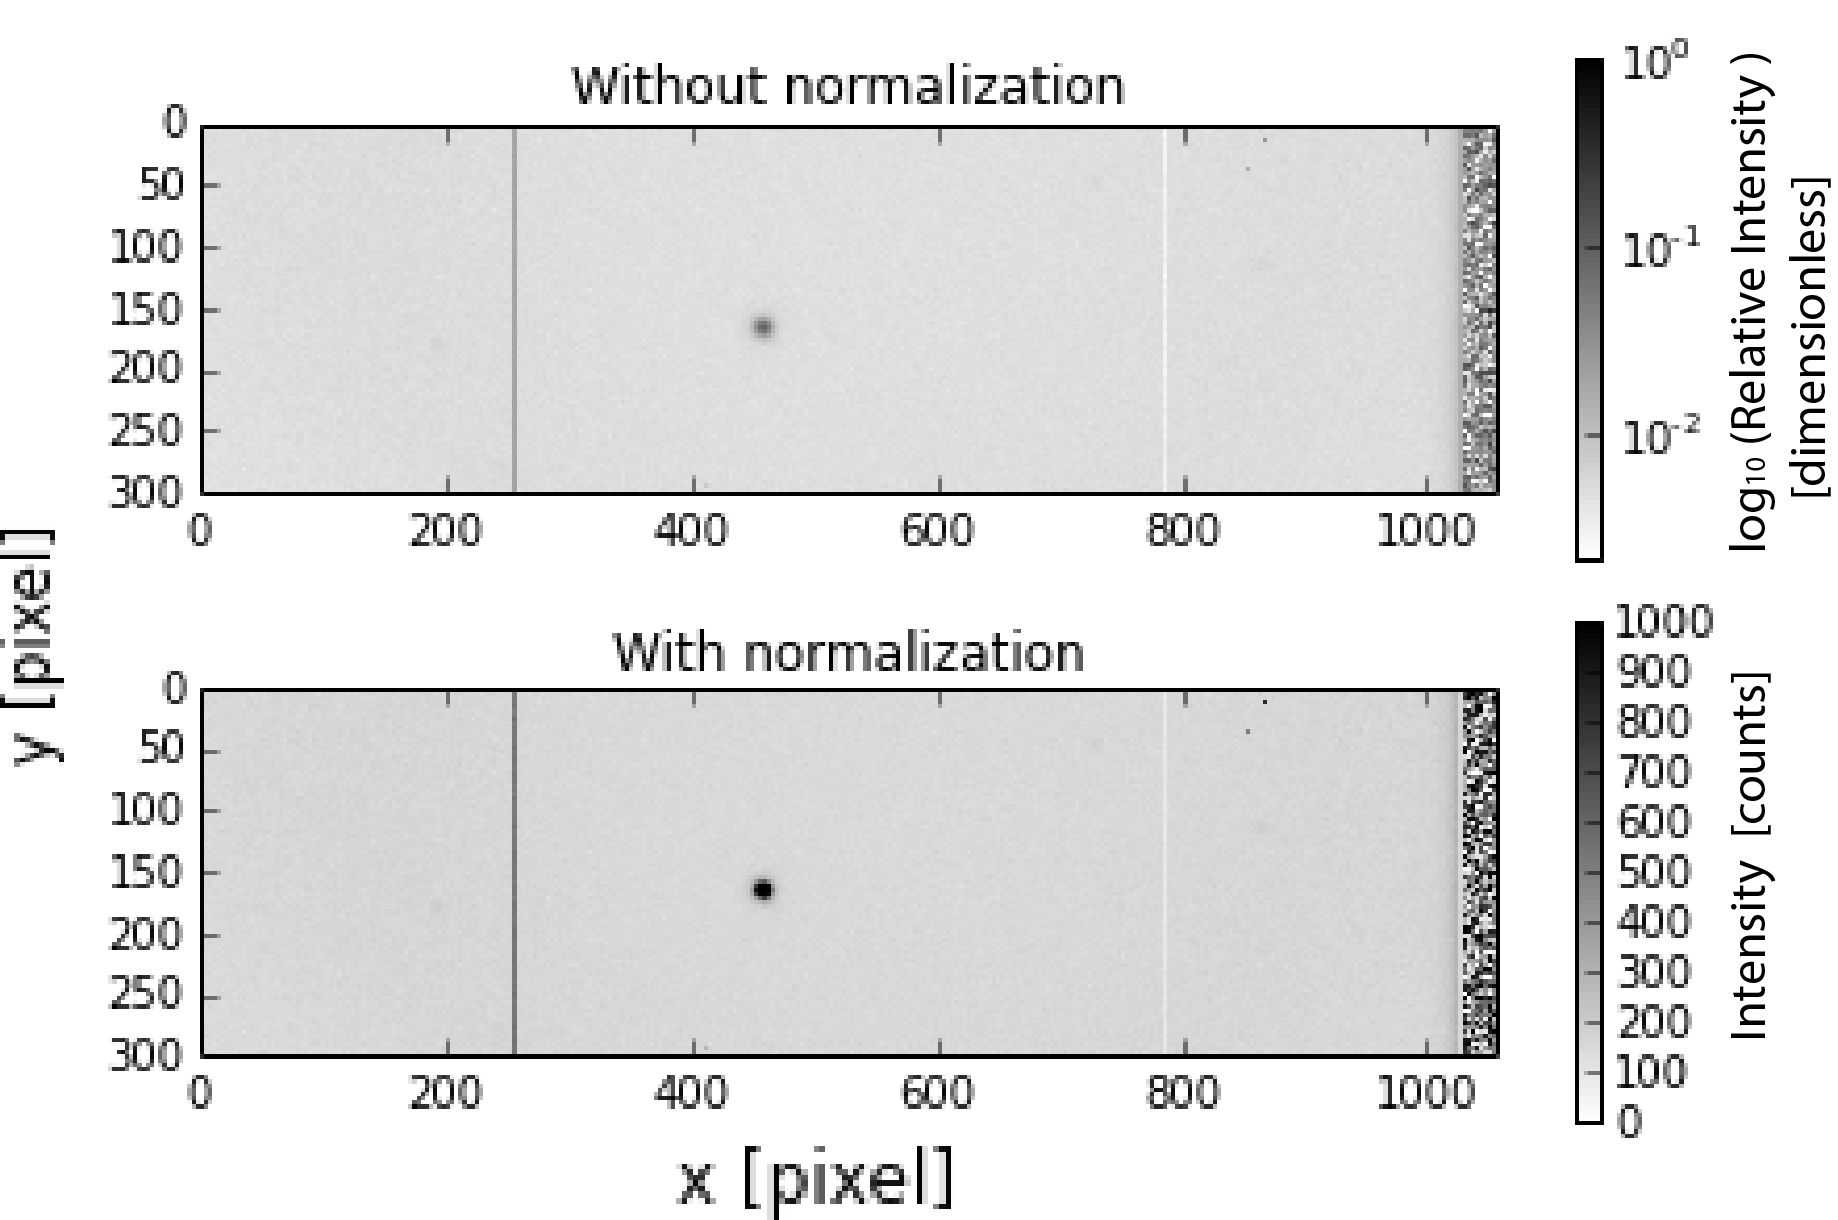
\includegraphics[width=0.5\textwidth]{figures/normalization}
\caption{Without normalization, the image requires a logarithmic stretch to distinguish the asteroid and the background since it has to accommodate for the range of decimal values resulted from the division. With normalization, the image can be viewed on a linear scale with a lower intensity limit of 0 and upper limit of 1000.}
\label{normalization}
\end{figure}
\subsection{Centroid-finding}
\label{centroid_find}
%intentionally adjust the Vmag lower cut than Vmag observed in NASA's small object dynamic so that it is able to identify the asteroid as a star.
In order to determine the positions of the stars on the image, we need to find the centroid position with the weight as the intensity value of each pixel. First, we set a threshold which was empirically adjusted to yield just enough stars for pattern recognition at around 3000 to 5000 counts, depending on the image. 
Since bad columns, corners, and borders often show up as completely dark pixels \footnote{Since image color scheme is inverted, the darkest pixel mean highest intensity.}, it is mistaken as a whole row of stars , we have to manually mask the pixels by zeroing the intensity value at the selected pixel.
	\begin{figure}[h!]
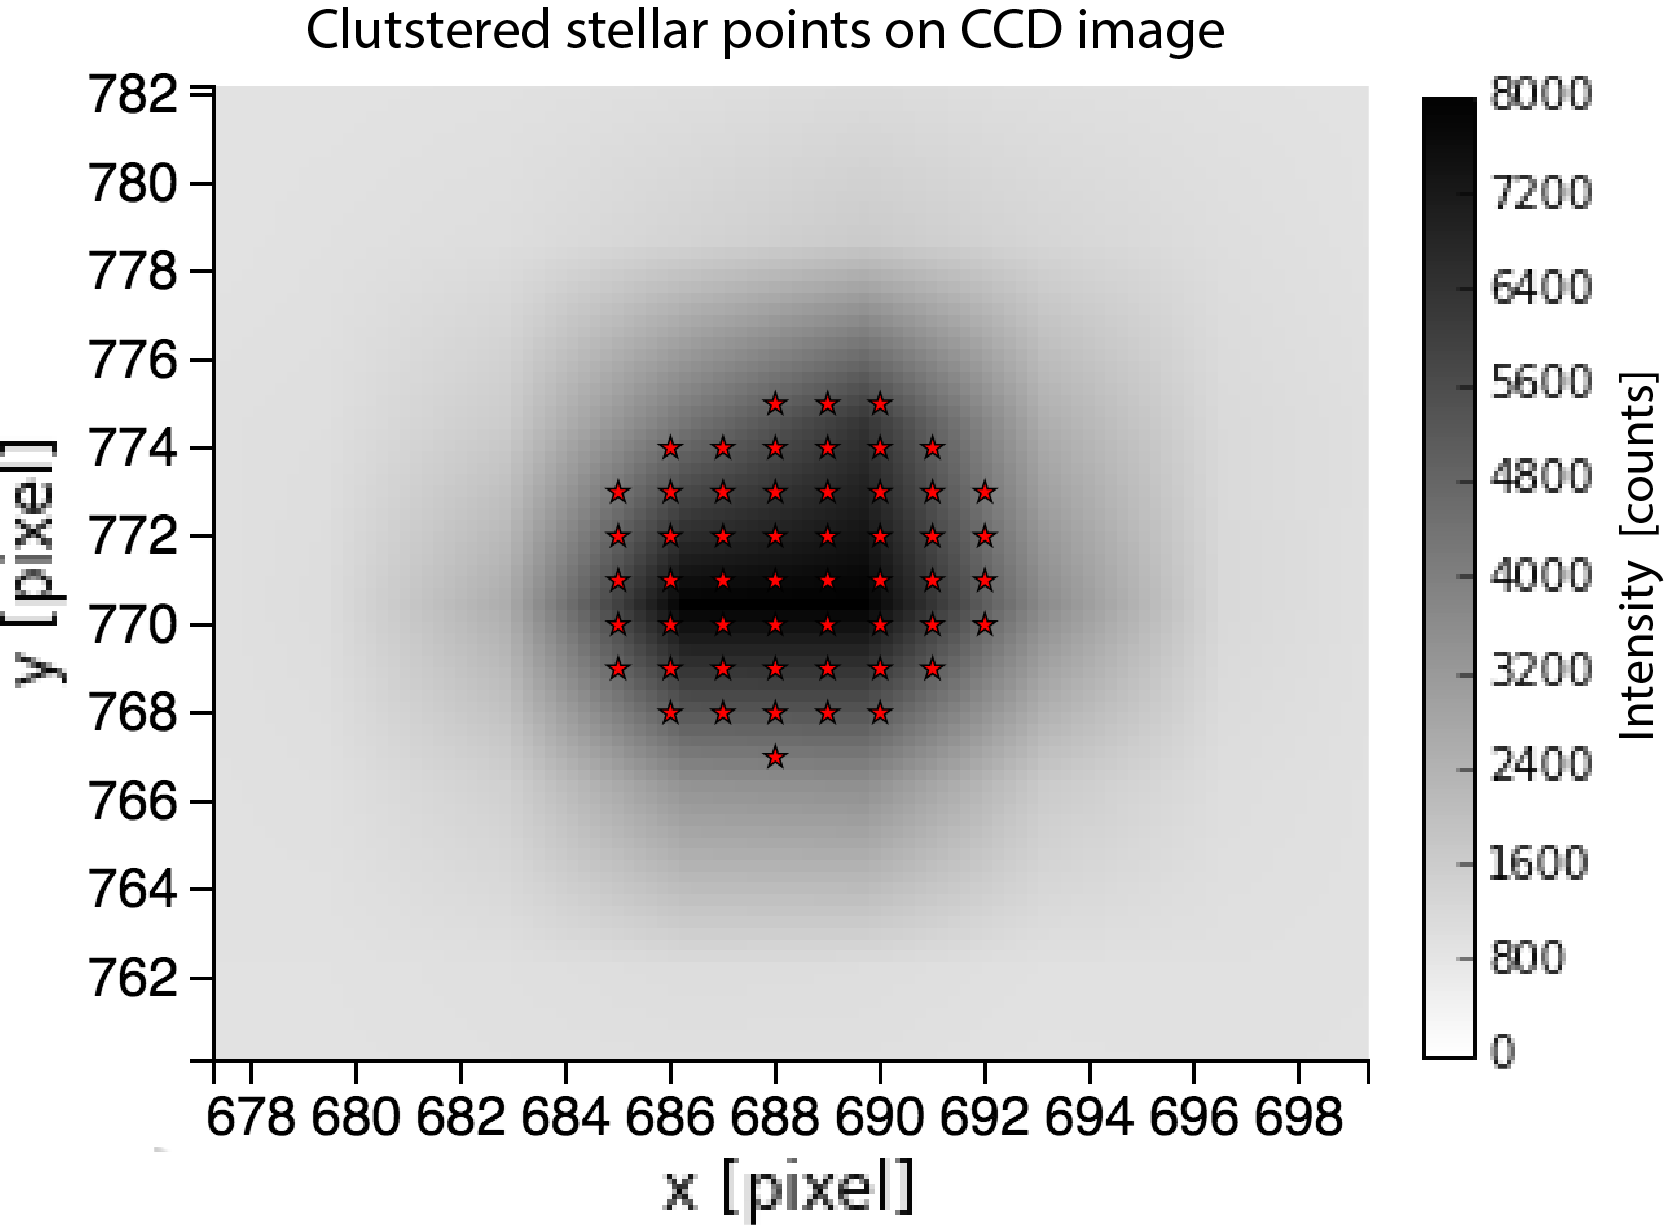
\includegraphics[width=0.5\textwidth]{figures/centroid_many}
\caption{A zoomed in image of a star and pixels that exceeds a threshold of 3000 counts belonging to the same star.}
\label{centroid_many}
\end{figure}
    	\begin{figure}[h!]
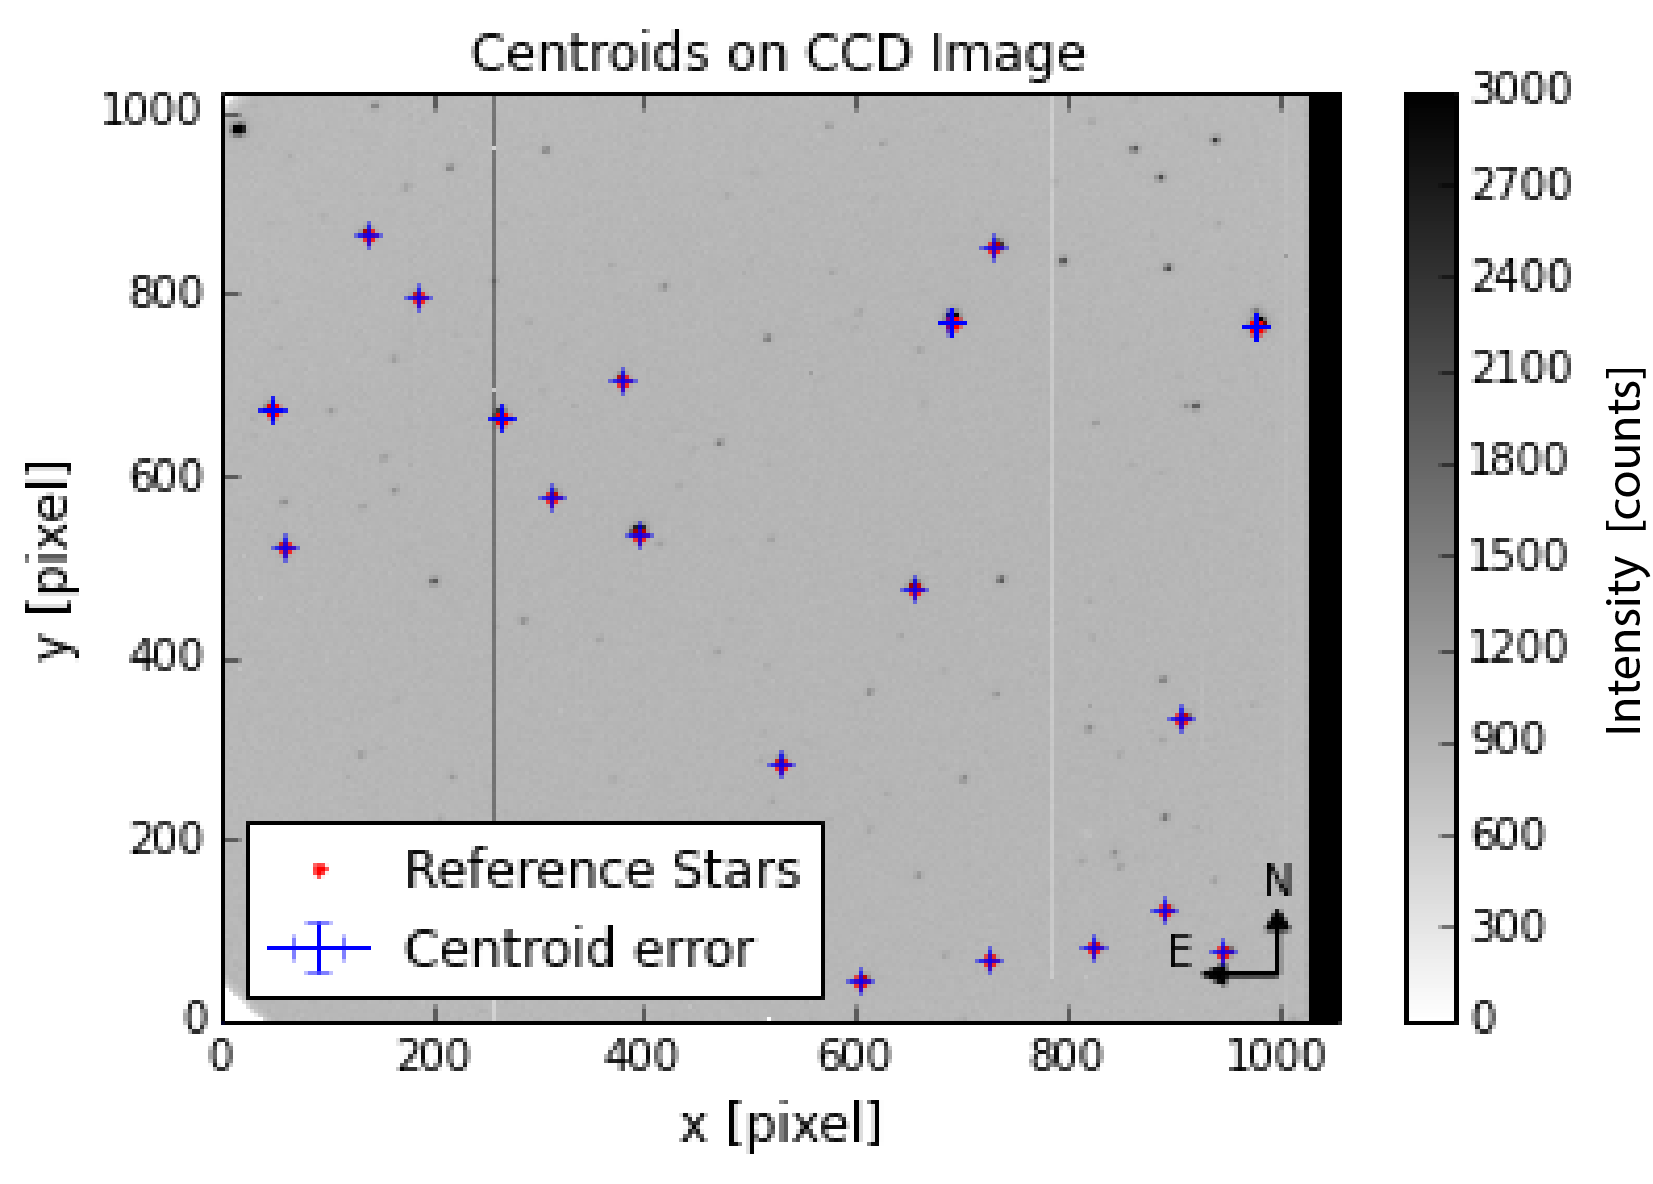
\includegraphics[width=0.5\textwidth]{figures/centroid_error_image}
\caption{Centroid computed for each star with plotted errorbar. Star pattern can be matched with the corresponding Aladin field as shown in Fig. \ref{aladin10162013}.}
\label{centroid_error_image}
\end{figure}
Since this is a fairly trivial case where the datapoints for each cluster is far apart, we use the more conceptually simplistic but computational intensive method of distance estimation instead of other clustering algorithm in the Machine Learning literature.  We loop through list of points above same threshold intensity and for every point we compute its pixel distance from another point in the same list. If the separation distance between two datapoints is less than 20 pixel, then it is clustered into the same group. Each cluster represent a star. This threshold intensity is intentionally chosen so that the asteroid can be mistakenly identified as a star. Now we have a list of pixel positions and intensity values of the datapoints that makes up a star, in order to get a representative value from cluster information, we compute centroid by Eq. \ref{centroid_eq} (From lab handout) :
\begin{equation}
\langle x\rangle = \frac{\sum \limits_{i} x_i I_i}{\sum\limits_{i} I_i}
\label{centroid_eq}
\end{equation}

\section{Astrometry}
Using stellar positions to calibrate the image
\subsection{Coordinate conversions on USNO stellar positions}\label{usno_coord_conv}
Since most reference stars are distant point sources, it is convenient to treat them as projected position onto a sphere centered at the observer. To match up and compare the stars on the CCD and the USNO stars in celestial coordinate, we must plot the USNO stars to pixel coordinates in the same coordinate system. In order to do so, we must first project celestial coordinates ($\alpha,\delta $) into standard Cartesian coordinates (X,Y) using Eq. \ref{projectionX} and 4 (From lab handout) : 
\begin{align}
X = -\frac{\cos(\delta) \sin(\alpha-\alpha_0)}{\cos(\delta_0)\cos(\delta)\cos(\alpha-\alpha_0)+\sin(\delta) \sin(\delta_0)}
\\ Y= -\frac{\sin(\delta_0)\cos(\delta)\cos(\alpha-\alpha_0)-\cos(\delta_0)\sin(\delta))}{(\cos(\delta_0)\cos(\delta)\cos(\alpha-\alpha_0)+\sin(\delta)\sin(\delta_0)}
\label{projectionX}
\end{align}
where ($\alpha,\delta $) are the (RA,DEC) for the USNO stars and ($\alpha_0,\delta_0$) are the center of the imaging field (i.e. the RA, DEC used to submit the USNO query\footnote{We were unable to use the RA, DEC given in the FITS header since it did not refer to the same sky location as what is shown on Aladin. Instead, we had to visually identify the star patterns in nearby region and set the center of the field position returned by Aladin and use those as our ($\alpha_0,\delta_0$) })
Then we use Eq.5 and \ref{scale_to_pix_coord} (From lab handout) to scale and offset the standard coordinate so that they are in pixel coordinate (x,y)  of Nickel's CCD camera. 
\begin{align}
x  = f \Bigg(\frac{X}{p}\Bigg)+x_0
\\ y  = f \Bigg(\frac{Y}{p}\Bigg)+y_0
\label{scale_to_pix_coord}
\end{align}
\begin{figure}[h!]
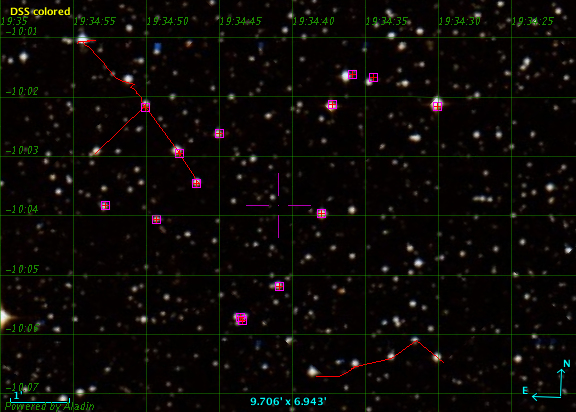
\includegraphics[width=0.5\textwidth]{figures/aladin10162013}
\caption{ Matching starfield pattern for October 16, 2013 with Aladin Sky Atlas, annotated to assist with  pattern recognition. Center crosshair position approximates the RA,DEC used in the USNO query. }
\label{aladin10162013}
\end{figure}

	\subsection{Least Square}\label{ls}
	\subsubsection{Objectives}\label{theory}
	The simple relation shown in Eq.5 and \ref{scale_to_pix_coord} does not factor in the possible shearing due to non-square pixels or rotation between standard Cartesian and the CCD's pixel coordinates. The goal of using the least square (LS) method  is to obtain the 6 plate constants in the first two rows of the transformation matrix \textbf{T} described by Eq. \ref{Tmatrix} (From Lab Handout): 
	\begin{equation}
\textbf{T}=	\begin{pmatrix}
(f/p)a_{11} & (f/p)a_{12} & x_0\\ 
(f/p)a_{21} & (f/p)a_{22} & y_0\\ 
0 &0  & 1
\end{pmatrix}
	\label{Tmatrix}
	\end{equation}
where $(x_0 , y_0)$are the telescope's pointing offset and f/p=561000 $\frac{\textrm{pixels}}{\textrm{radian}}$. 
The value of the plate constants $a_{ij}$ results from a combination of scale, shear,translation, and rotation operations on the input image. \textbf{T} provides a linear mapping between pixel space  \textbf{x} and standard Cartesian space \textbf{X}. By adopting matrix notations, we can condense N equations of condition for all the positions found in Sec.\ref{scale_to_pix_coord} into one single matrix equation \textbf{a}=\textbf{Bc} where: 
\begin{align}
\label{aBc}
\textbf{a}= \begin{bmatrix}
 x_1
\\ x_2
\\:
\\:
\\x_N
\end{bmatrix}
\quad
\textbf{B}=\Bigg(\begin{smallmatrix}
(f/p)X_1 & (f/p)Y_1  & 1\\ 
(f/p)X_2  & (f/p)Y_2  & 1\\ 
: &:  &: \\ 
(f/p)X_N  &(f/p)Y_1   & 1
\end{smallmatrix}\Bigg)
\\
\textbf{c} = \begin{pmatrix}
a_{11} & a_{12} & x_0 
\end{pmatrix}
\end{align}
		In order to compute the plate constants, we select the best-fitting model by using LS to choose the parameters in our model that yields the smallest error for the given set of position data. Therefore by minimizing the sum of all the squares of the residuals $\chi^2$=$\|\textbf{a}-\textbf{Bc}\|^2_{\tiny{2}}$ , we can compute the best-fitting plate constants in $\textbf{c}$ as shown in Eq. \ref{c_eq}:
		\begin{equation}
		\textbf{c} = (\textbf{B}^T\textbf{B})^{-1}\textbf{B}^T\textbf{a}
		\label{c_eq}
		\end{equation}
			
	\subsubsection{Implementation and Results}
	The steps in the pixel-to-celestial conversion is implemented in a reverse order than how it is intuitively explained in Sec. \ref{theory}. First, we construct the matrices \textbf{a}, \textbf{B}, \textbf{c} described by Eq.\ref{aBc} and 9, and substituting the \textbf{a}$_x$ and \textbf{c}$_x$ notation for \textbf{a} and \textbf{c}. \textbf{a}$_x$ is a list of USNO stellar x pixel positions converted from celestial to pixel coordinates described in Sec. \ref{scale_to_pix_coord}.  \textbf{B} is constructed using the USNO's X and Y standard coordinate positions projected by Eq.\ref{projectionX} and 5. Then we use Eq.\ref{c_eq}
to get the first 3 plate contant ($a_{11}\quad a_{22}\quad x_0$) in \textbf{c}$_x$	. Similarly, we construct $a_y$ from the y positions and implement the same procedure to solve for $c_y=(a_{21} \quad a_{22}\quad y_0)$.
Using the 6 plate constants, we can now construct the matrix \textbf{T} and map a list of pixel coordinates from the CCD image stars to celestial coordinates by left multiplying pixel coordinates with \textbf{T}$^{-1}$. Finally, the RA, DEC of the stellar positions is obtained from performing the standard-to-celestial coordinate projection using Eq. \ref{tan_proj} and \ref{sin_proj} (From Lab Handout):
\begin{equation}
\tan(\alpha-\alpha_0)=-\frac{X}{\cos\delta_0-Y\sin\delta_0}
\label{tan_proj}
\end{equation}
\begin{equation}
\sin \delta= \frac{\sin \delta_0+Y\cos\delta_0}{(1+X^2+Y^2)^{1/2}}
\label{sin_proj}
\end{equation}
where $(\alpha,\delta)$ is the (RA,DEC) in celestial coordinates and $(\alpha,\delta)$ is the (RA, DEC) at the center of the image.
 As plotted in Fig.\ref{starfield_match} the list of stars should also include the coordinate of asteroid, which was intentionally misidentified as a star since the same procedure is conducted in the same manner in Sec. \ref{centroid_find}. 
%	The offset value is adjusted after conducting least square using first the standard ($x_0,y_0$)  first identifying matching pairs of stars from USNO and CCD image, then calculate the distance between them using the Pythagoras theorem. The distance is an offset that can be added to all the data points to precisely match the two datasets, or simlarly  for the initial $(x_0, y_0)$ with the addition.
	\begin{figure}[h!]
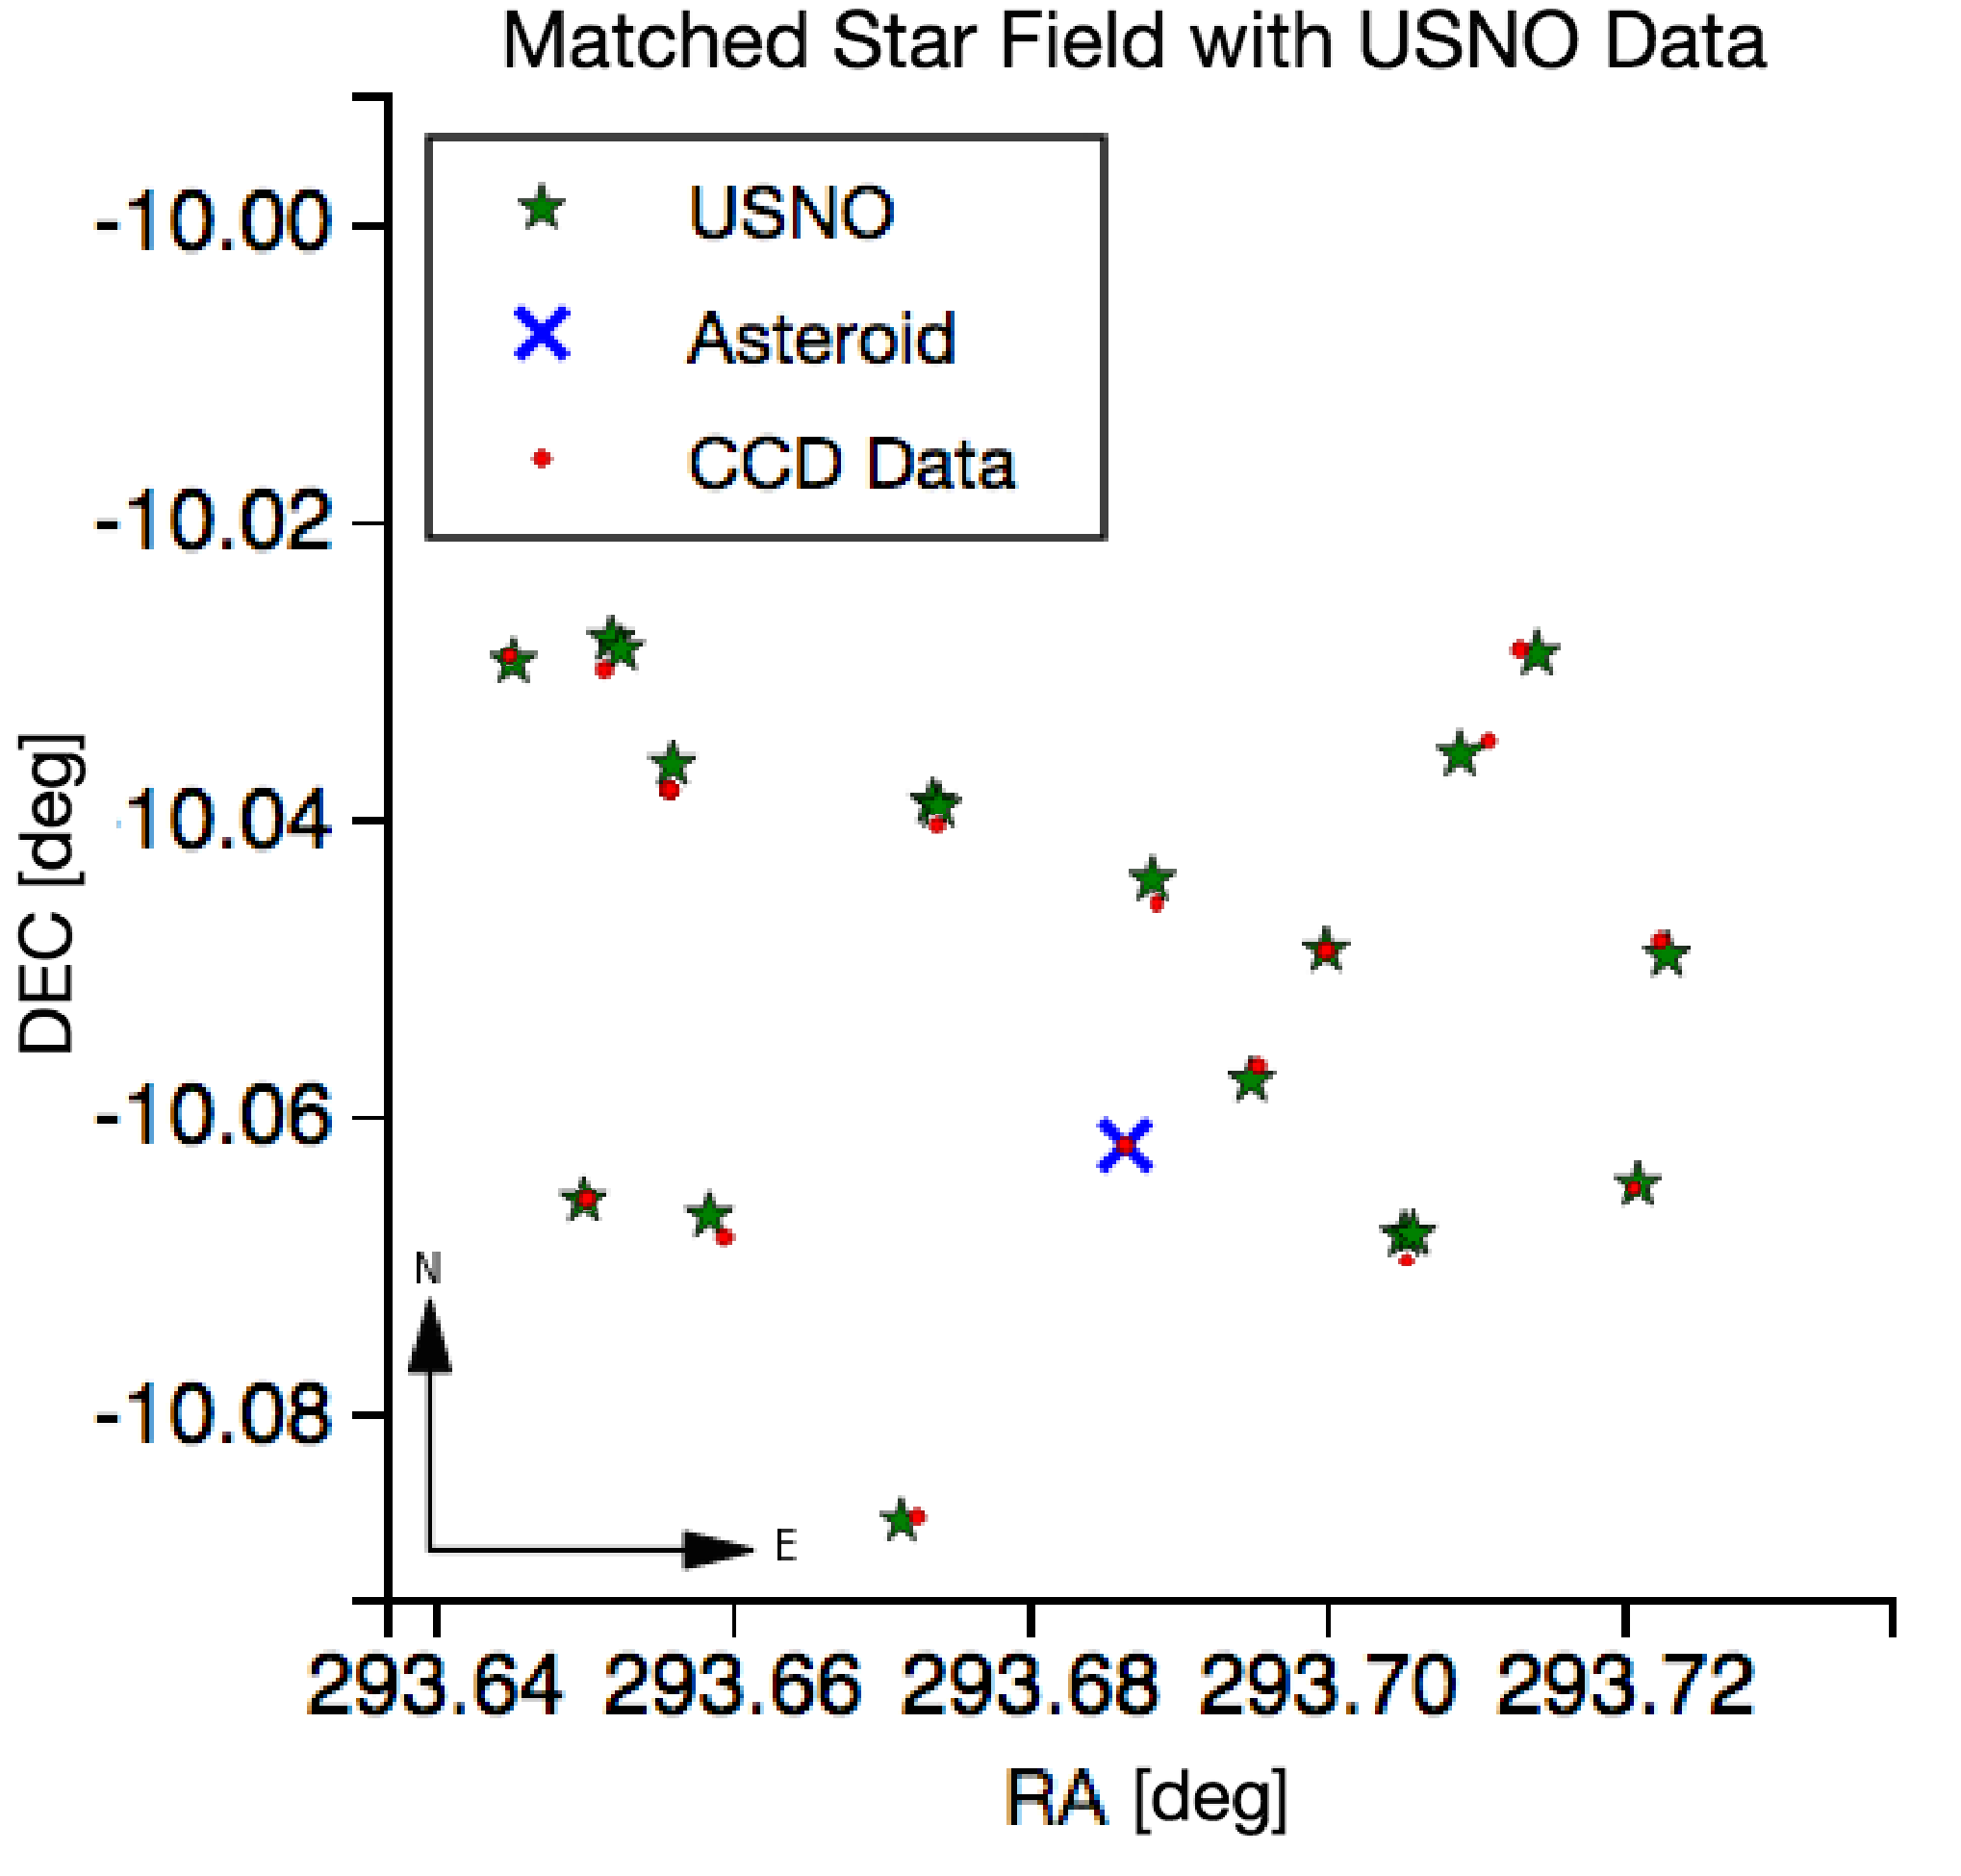
\includegraphics[width=0.5\textwidth]{figures/starfield_match}
\caption{ Matching starfield with USNO-B1 of bright stars $<$ 14.4 mag for October 16, 2013. The asteroid is easily identified as it shows up on the CCD image but not on the USNO-B1 catalog.}
\label{starfield_match}
\end{figure}
%Since the model we used for least square is a linear ---- with its intercept set as zero, we don't minimize the offset parameter. parameter has no offset (translation). We need to manually ---. Alternatively we could have also come up with a model that also minimized the offset. 
We find that the final projected image in celestial coordinates is horizontally flipped compared to the the our CCD image (Fig.\ref{centroid_error_image} ) and  Aladin Sky Atlas (Fig.\ref{aladin10162013}) because for a celestial observer looking up at the sky, North up points behind the observer so his right side points in the eastward direction.

%Position vector can be obtained from the HORIZONS Web-Interface 

%This could be verified with the vector from earth to asteroid.

    \subsection{Iterative solution}
    We conduct the all procedures mentioned in the above sections to the night of Oct 16, 17, 20, and 21. Only 3 epochs are necessary for computing the distance. We can not use the same transformation matrix \textbf{T} for every night even though the imaging is done on the same telescope with the same magnification and shear, the rotation and offset will cause the plate constants to differ. Following Eq.\ref{dx_defn} (Stewart, pg.174) , we chose the 3 of the closest nights (16,17,20)  in order to minimize the interval that we are computing our time derivative over to get as close to $\lim_{h\rightarrow 0}$ of the derivative definition as possible.
\begin{equation}
f'(x) = \lim_{h\rightarrow 0}\frac{f(x+h)-f(x)}{h}
\label{dx_defn}
\end{equation}
where h is an infinitesimal interval of x. Before proceeding to using the positions of the asteroids at 3 epochs to find  asteroid's distance, we plotted the coordinates of the asteroid as a sanity check as shown in Fig. \ref{motion_path}.
\begin{figure}[h!]
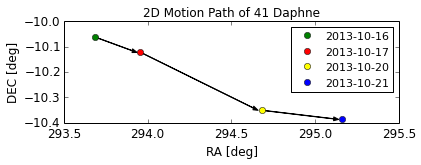
\includegraphics[width=0.5\textwidth]{figures/motion_path}
\caption{The minor deviation from the straight motion path caused by supressing the 3D orbital of the asteroid onto the 2D plot and could be explained by the asteroid's motion in the other directions. As shown in the JPL emphemeris velocity vectors, even though the $V_y$ is much larger than $V_x$ and $V_z$, $V_x$ and $V_z$ are still non-zero.}
\label{motion_path}
\end{figure}

    Using the RA, DEC positions of the asteroid, we can construct the unit vectors ($\vec{s_1},\vec{s_2},\vec{s_3}$) that points from Earth to the asteroid for each of the 3 nights: 
    \begin{equation}
    \vec{s}=\begin{pmatrix}
\cos\alpha\cos\delta\\
\sin\alpha\cos\delta 
\\ \sin \delta
\end{pmatrix}
    \end{equation}
 By querying JPL Horizon  using the datetime given in the FITS header of the October 17, 2013 exposure, we can construct the heliocentric vectors to Earth ($\vec{R}$). JPL horizon by default returns the ecliptic coordinate, so we must change the interface setting so that returned the Earth-to-Sun vector is in equatorial coordinates to conform with the more convientient coordinate system for describing orbital motion. Otherwise, this would affect the values for y and z components of the position (and velocity) vector returned since in the ecliptic system the  xy-plane is spanned by  Earth's mean equator at the reference epoch.
    
    The reason why we need exposures from two other epochs is that  $s_1$ and $s_3$ vectors are used in the Taylor approximations of the $s_2$ time derivatives as shown in Eq. \ref{ds} and \ref{dds} (From Lab Handout).
    \begin{equation}
    \dot{s_2} =\frac{\tau_3(s_2-s_1)}{\tau_1 (\tau_1+\tau_3)}+\frac{\tau_1(s_3-s_2)}{\tau_3(\tau_1+\tau_3)}
    \label{ds}
    \end{equation}
    \begin{equation}
      \ddot{s_2} =\frac{2(s_3-s_2)}{\tau_3 (\tau_1+\tau_3)}-\frac{2(s_2-s_1)}{\tau_1(\tau_1+\tau_3)}
    \label{dds}
    \end{equation} 
    By plugging in the obtained vectors and substituting $\vec{s}$ for $\vec{s_2}$ in the dynamical equation governing the Newtonian two body problem in the center-of-mass rest frame, we get the scalar value results in Eq. \ref{p}.
    \begin{equation}
    \rho = k^2\Bigg(\frac{1}{R^3}-\frac{1}{r^3}\Bigg)\frac{\dot{s}\cdot(\vec{R}\times \vec{s})}{\dot{s}\cdot(\ddot{\vec{s}}\times\vec{s})}
    \label{p}
    \end{equation}
    where $\rho$ is the scaling factor for $\vec{s}$ that can be used to find the distance to asteroid\footnote{Since unit vectors are by normalized by its own magnitude, it is by definition dimensionless. Therefore, to construct physical units in the Earth-Asteroid vector, $\rho$ must have units of AU.}
    r is the sun-asteroid distance and R is the sun-Earth distance (computed from the norm of their respective vectors) and k = $\sqrt{GM_{sun}}$ in Gaussian units.
    Along with the laws of cosine,  we have two coupled equation with two unknowns  $\rho$ and r describing the orbital situation.
    \begin{equation}
    r^2 = \rho^2+R^2+2\rho \vec{R}\cdot\vec{s}
    \label{r}
    \end{equation}
     By providing a reasonable initial guess of 3 AU, we iteratively solve for $\rho$ by plugging in the result returned from Eq.\label{r} to Eq.\ref{p} and vice versa. The system of equation converges in each step of the iteration because in order to solve it you must have values that satisfy each either the r or $\rho$ equation. Therefore, the possible values for the solution is rapidly constrained at each step as this is a cubic equation. The convergence of the resulting $\rho$ as shown in Fig.\ref{convergence_example} is a sign that the solution simultaneously satisfy both equations. 
    \label{iterative_soln}
    	\begin{figure}[h!]
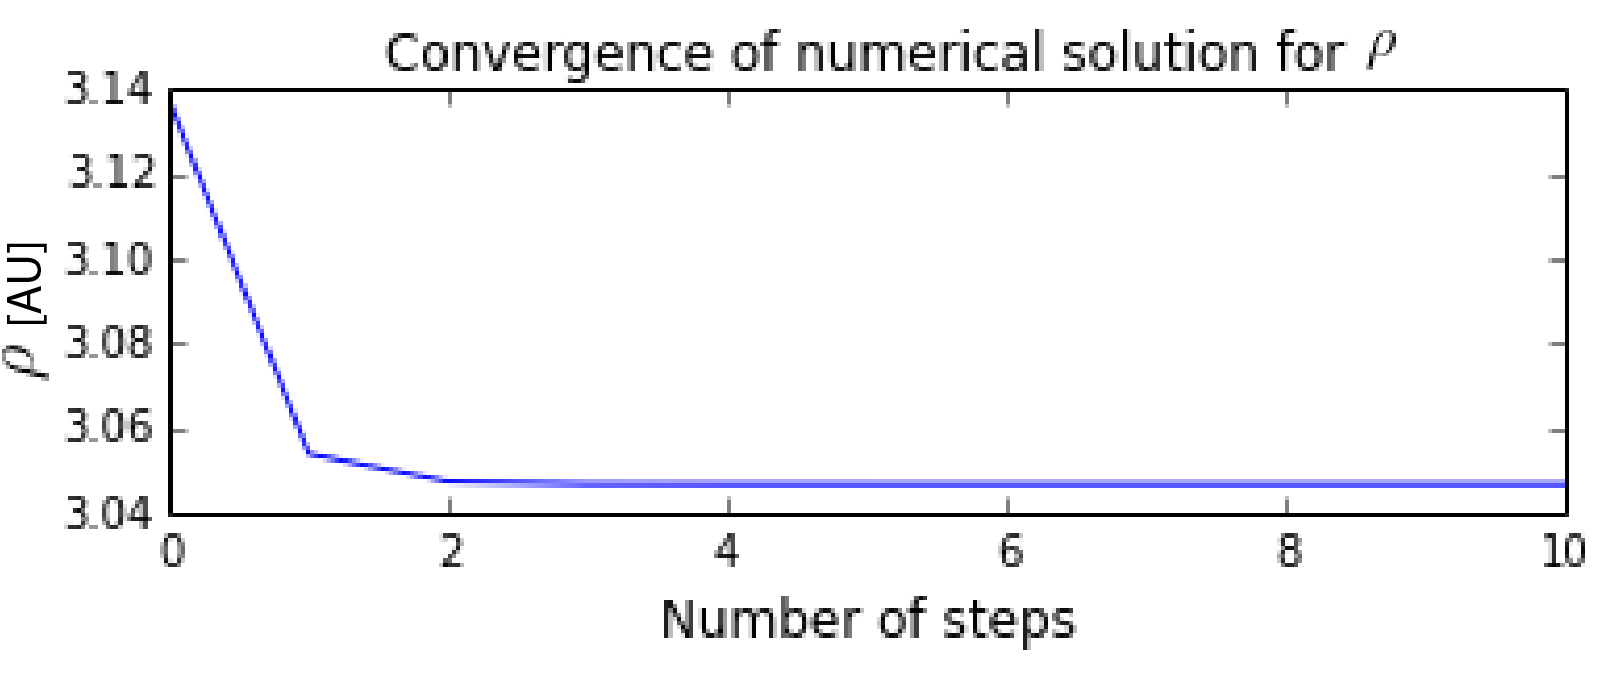
\includegraphics[width=0.5\textwidth]{figures/convergence_example}
\caption{ By conducting this procedure for 1000 times with slightly varied input values as described in Sec.\ref{monte_carlo}, we find that the solution takes an average of 5 steps to converge as shown in the graph above  (where we arbitrarily define a solution as ``converging" when the difference between solutions at consecutive steps is less than 1.0$\times10^{-5}$AU). It is interesting to note that each step brings the computed result closer to the actual solution by approximately an order of magnitude. }
\label{convergence_example}
\end{figure}
  
Since the vector $\rho \vec{s}$ subtends from the Earth to asteroid, the norm of  $\rho \vec{s}$ yields a distance of 3.047 AU from Earth to 41 Daphne on the night of October 17, 2013, which has a 19\% percent difference from the values returned by NASA Solar System Bodies web tools. The possible source of error  contributing to the deviation from the nominal value is discussed in the next section. 
\section{Error and Uncertainty}
\subsection{Centroid Error}
\label{centroid_error}
In order to find the error on the value of $\rho$ that scales the Earth-to-asteroid distance, we must first determine the error on the centroid values used to find $\rho$. 
By assuming that the error on each pixel is uncorrelated, we can apply the method of error propagation on Eq. \ref{centroid_eq} and obtain:
\begin{equation}
\sigma^2_{<x>}=\sum_{i} \Bigg(\frac{\partial \langle x\rangle}{\partial I_i}\Bigg)^2
\label{error_prop_centroid}
\end{equation} 
Computing $\frac{\partial \langle x\rangle}{\partial I_i}$ and plugging it back into Eq. \ref{error_prop_centroid}: 
\begin{equation}
\sigma^2_{\langle x\rangle}=\frac{\sum\limits_{j}I_j (x_j-\langle x\rangle)^2 }{\Big(\sum \limits_{i} I_i\Big)^2}
\end{equation}

Using the list of clustered star position as described in Sec. \ref{centroid_find}
The same method is also used to calculate the error on <y> 
However this obtained results is in units of pixels, we must convert this error to units of degree as shown in Fig.\ref{uncertainty_range} 
    	\begin{figure}[h!]
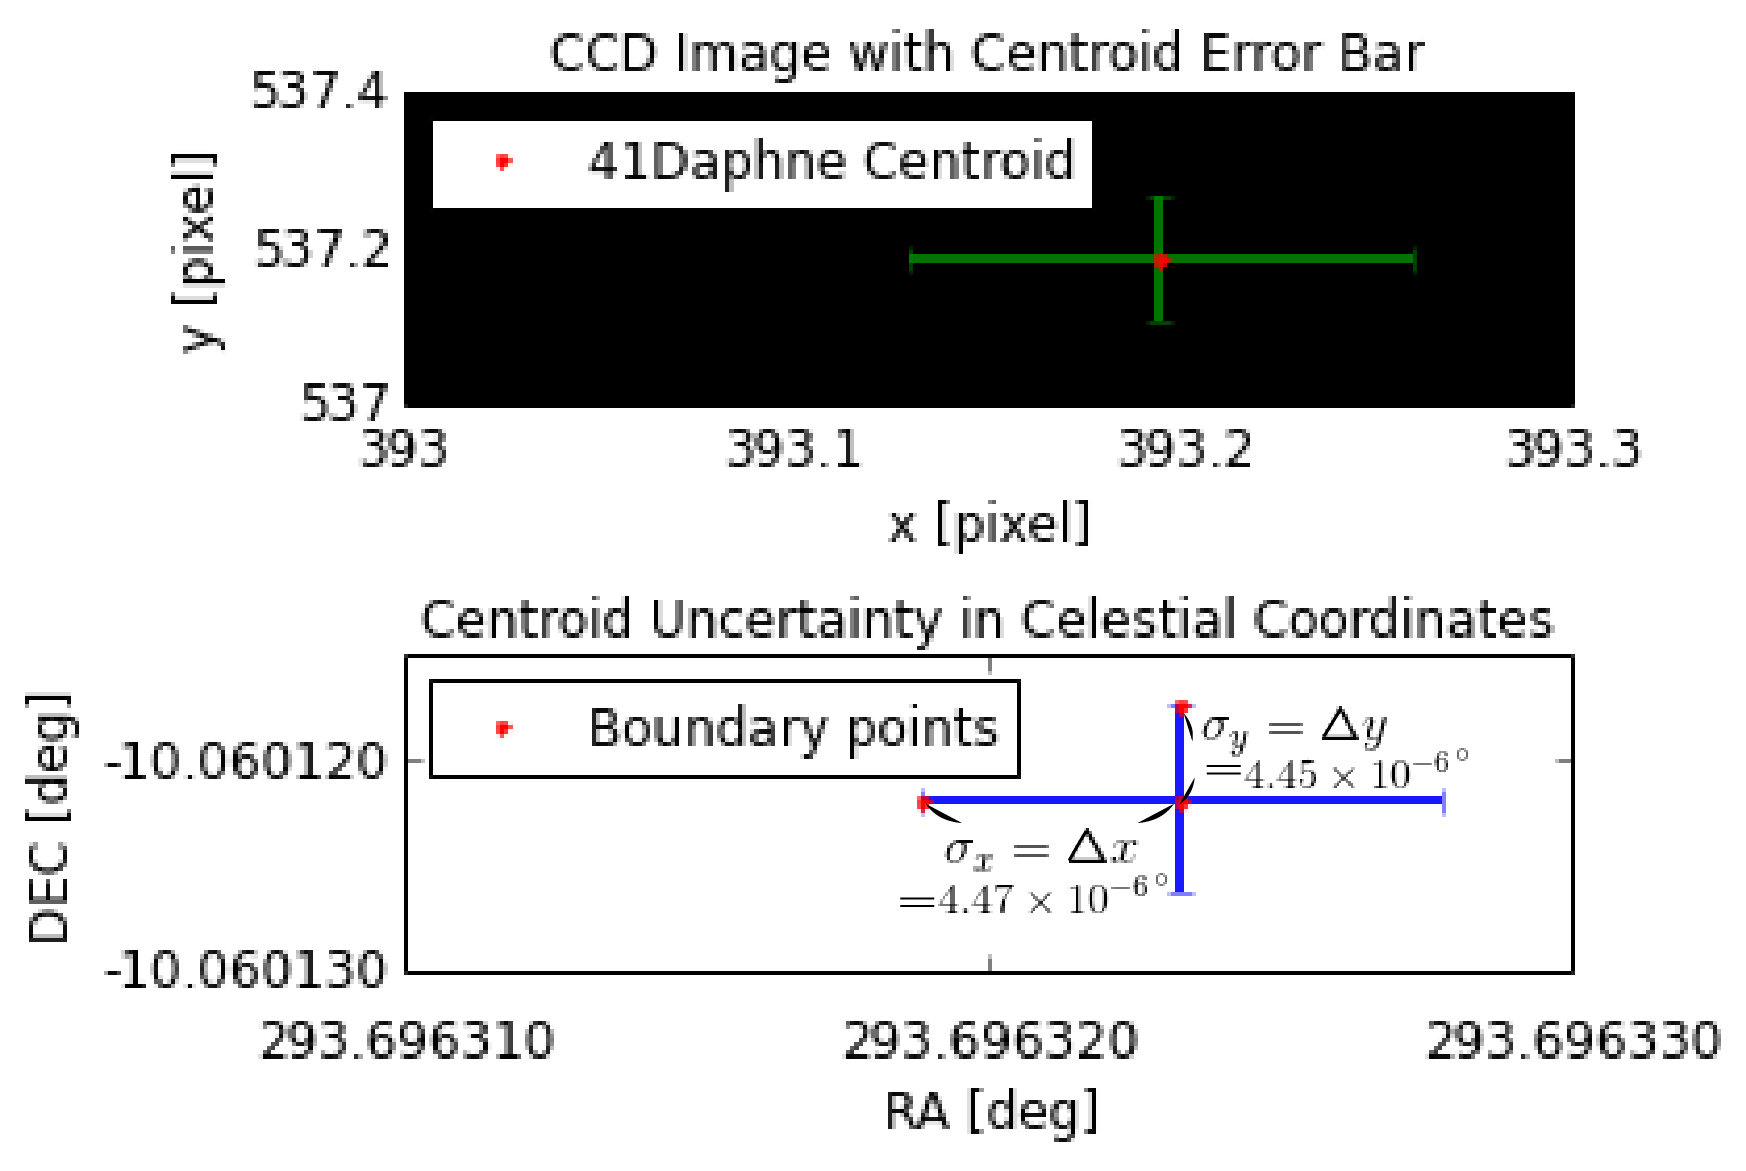
\includegraphics[width=0.5\textwidth]{figures/uncertainty_range}
\caption{ Since the pixel-to-celestial coordinate conversion procedure described in Sec. \ref{ls} transforms coordinates rather than interval values. We select two boundary points that defines where the x and y error bar subtends and convert these to celestial coordinates. Then subtracting boundary points from the asteroid's centroid position in celestial coordinates, we obtain the x and y uncertainty ranges ($\sigma_x,\sigma_y$) in units of degrees, which has a value of around 0.016 arcseconds.}
\label{uncertainty_range}
\end{figure}

\subsection{Monte Carlo Method}
\label{monte_carlo}
Since we do not have an analytical solution to solve for $\rho$ we can not compute the partial derivatives used in the error propagation equation. Instead we use the Monte Carlo method to approximate the error on our obtained value of $\rho$ given the centroid error of the asteroid's celestial position. First, we construct two Gaussian nosie distribution with standard deviation as the x and y centroid error that we obtained in Sec. \ref{centroid_error}. Then we draw a random value from each distribution to construct a noise vector for the x,y component with the noise on the z component set as zero.\footnote{ We have no information about the error on z  because it is not involved in the centroid-finidng calculations. Since the CCD image is 2D, we can only compute the centroid error along x and y component.}  The noise vector is added to $\vec{R}$ and this newly computed $\vec{R}$ is used in the iterative algorithm to compute the solution for $\rho$ as described in Sec.\ref{iterative_soln} with other parameters kept the same. The Gaussian distribution is centered at zero so that the random noise may be positive or negative. This ensures that the computed $\rho$ solutions are not skewed to  a higher value by the addition of the noise vector. By performing the Monte Carlo procedure on 100000 trials, the standard deviation of the list of computed $\rho$ values yields the approximate error on the value of $\rho$. As shown by conducting this procedure on different number of trials from $10^3$ to $10^6$, the choice of using 1$\times10^5$ trial is sufficiently large enough so that the standard deviation result does not vary by a lot relative to a choice of 1$\times10^6$ or more.
    	\begin{figure}[h!]
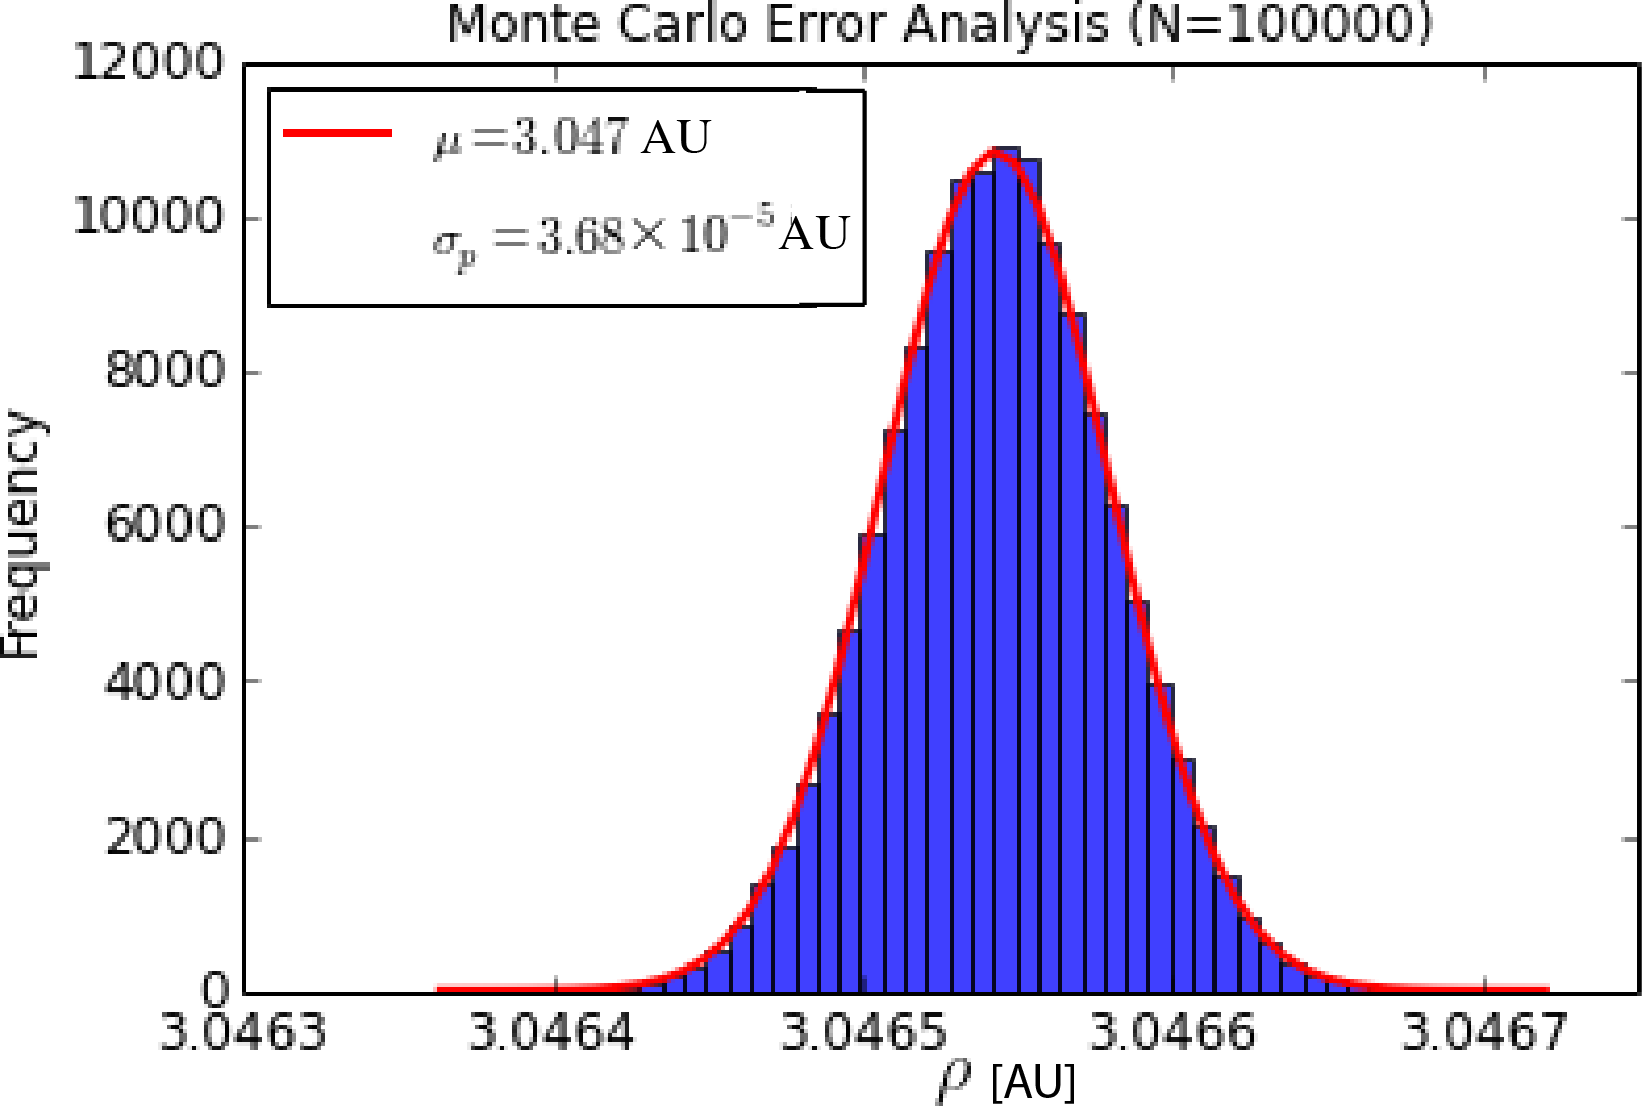
\includegraphics[width=0.5\textwidth]{figures/monte_carlo_result}
\caption{The standard deviation on this Gaussian distribution approximates the error on $\rho$ to be $3.68\times10^{-5}$ AU ($\approx$ 5505 km).}
\label{monte_carlo_result}
\end{figure}
\subsection{Other possible error contribution}
The error computed from the Monte Carlo method certainly doesn't add to the 0.48 AU deviation from the values returned by NASA's small body simulation. Other error terms may be a result of truncating  higher order terms when approximating the velocity and acceleration for $\vec{s}$ as the average interval of h in Eq. \ref{dx_defn} is approximately 1 and 3 days. 

In addition,  we only examined errors on the asteroid position. However, uncertainty in the measurement of stellar position can also affect our asteroid position result since stellar positions are treated as the ``data" in our best-fit model when conducting the least square procedure. This propagates to uncertainty on the plate constant values used in the conversion from pixel to standard coordinates. Nevertheless, this effect should be secondary to the ones we directly computed for the asteroid. 
\section{Conclusion}
In this experiment, we collect images of the asteroid 41 Daphne at 3 different epochs from the Nickel telescope at Lick Observatory for finding distance to the asteroid. We apply dark, flat, and bias corrections to the images to make the CCD signal linearly proportional to the astronomical source. We devise an algorithm that clusters the pixels that belong to the same star and use that information find the centroid positions of stars in the image field. Using the method of error propagation, we obtain an closed-form expression that enables us to compute the uncertainty on the obtained centroid positions. 

Using the method of least square on the USNO stellar positions, we obtain a transformation matrix that maps from standard Cartesian to pixel coordinates. Applying the inverse of this matrix to the CCD pixel positions of the centroid, we can obtain their positions in standard coordinates which can then be projected to celestial coordinates. By matching together stars from the USNO-B1 catalog and our CCD image, we can figure out which identified star is actually the asteroid of interest. Using the heliocentric vector to Earth returned by JPL Horizon for the time when the exposure is taken, along with the celestial coordinates of the asteroid computed from the conversion, we iteratively solve for two coupled equations relating $\rho$ and r. The iterative algorithm numerically computed that 41 Daphne is approximately 3.047 AU away from us on the night of October 17,2013. As we do not have an analytical solution to finding $\rho$, we instead used the Monte Carlo method to numerically propagate the error on the obtained distance and approximate the error to be $3.68\times10^{-5}$ AU.

As we only  determine the distance to the source in this lab,, one possible extension to this project is to find all the Keplerian orbital elements describing the orbital motion of 41 Daphne. This calculation can be done with just the three epochs of imaging data and astrometric information obtained from this lab. Moreover, the distance information obtained in this lab is value is useful for approximating other physical properties that characterize an astronomical body such as its luminosity, mass and size.
 \section*{References}

 \begin{footnotesize}
 \begin{itemize}
\item Howell, Steve,  \textit{Handbook of CCD Astronomy}, 2nd Edition. Cambridge University Press, 2006.
%\item Wall, J. V. and Jenkins, C.R., \textit{Practical Statistics for Astronomers}, Cambridge University Press, 2002.
%\item Press, William H., and William T. Vetterling. \textit{Numerical Recipes in C: The Art of Scientific Computing}. Cambridge University Press, 1992. 
\item Chromey, Frederick R. \textit{To Measure the Sky: An Introduction to Observational Astronomy}. Cambridge: Cambridge UP, 2010. Print.
\item Stewart, James. \textit{Calculus: Early Transcendentals}. 7th ed. Belmont: Thomson/Brooks/Cole, 2003. Print.
\item Perryman, M.A.C. and Lindegren, L. and Kovalevsky, J. and Hoeg, E. and Bastian, U. and Bernacca, P.~L. and Cr{\'ez\'e}, M. and Donati, F. and Grenon, M. and Grewing, M. and van Leeuwen, F. and van der Marel, H. and Mignard, F. and Murray, C.A. and Le Poole, R.S. and Schrijver, H. and Turon, C. and Arenou, F. and Froeschl{\'e}, M. and Petersen, C.S.. The HIPPARCOS Catalogue. . p. L49-L52 1997
\item  Lindegren, L. and Babusiaux, C. and Bailer-Jones, C. and Bastian, U. and Brown, A.G.A. and Cropper, M. and Hog, E. and Jordi, C. and Katz, D. and van Leeuwen, F. and Luri, X. and Mignard, F. and de Bruijne, J.H. J. and Prusti, T.. The Gaia mission: science, organization and present status. . p. 217-223 2008
\end{itemize}
% \bibliography{references}
%\bibliographystyle{elsarticle-harv}
  \end{footnotesize}

\end{document}
